\documentclass{article}

\usepackage{fancyhdr, lastpage}
\usepackage[inline]{enumitem}
\usepackage{listings}
\usepackage[scaled=0.95]{inconsolata}  % Use a monospaced font, like Inconsolata
\usepackage{wasysym}
\usepackage{booktabs}
\usepackage{multicol}
\usepackage{siunitx}
\usepackage{xfrac}
\usepackage{extramarks}
\usepackage{amsmath, amsthm, amsfonts, mathtools,}
\usepackage{caption}
\usepackage{xcolor}
\usepackage{tikz,tcolorbox}


% Define MATLAB code style
\lstdefinestyle{matlabstyle}{%
  language=Matlab,
  basicstyle=\ttfamily\small,    % Use a smaller font
  keywordstyle=\color{blue},
  commentstyle=\color{green!40!black},
  stringstyle=\color[RGB]{167, 9, 245},
  numbers=left,
  numberstyle=\tiny,
  numbersep=5pt,
  frame=single,
  breaklines=true,
  breakatwhitespace=true,
  captionpos=b,
  morekeywords={matlab2tikz},
  showstringspaces=false,
}

% MATLAB Code Example

% \begin{lstlisting}[style=matlabstyle, caption={Your MATLAB code here}]
%     % MATLAB code goes here
%     function output = myFunction(input)
%         % Comment
%         output = input + 1;
%     end
%     \end{lstlisting}

% Change Text Color Example

% This is \textcolor{red}{red} text.
% \textcolor{blue}{This is blue text.}
% \textcolor{green!50!black}{This is green text.}

%
% Basic Document Settings
%

\topmargin=-0.45in
\evensidemargin=0in
\oddsidemargin=0in
\textwidth=6.5in
\textheight=9.0in
\headsep=0.25in

\linespread{1.1}

\pagestyle{fancy}
\lhead{\hmwkAuthorName}
\chead{\hmwkTitle}
\rhead{\hmwkClass}
\lfoot{\lastxmark}
\cfoot{Page \thepage\ of \pageref{LastPage}}

\renewcommand\headrulewidth{0.4pt}
\renewcommand\footrulewidth{0.4pt}

\setlength\parindent{0pt}

%
% Create Problem Sections
%

\newcommand{\enterProblemHeader}[1]{
    \nobreak\extramarks{}{Problem \arabic{#1} continued on next page\ldots}\nobreak{}
    \nobreak\extramarks{Problem \arabic{#1} (continued)}{Problem \arabic{#1} continued on next page\ldots}\nobreak{}
}

\newcommand{\exitProblemHeader}[1]{
    \nobreak\extramarks{Problem \arabic{#1} (continued)}{Problem \arabic{#1} continued on next page\ldots}\nobreak{}
    \stepcounter{#1}
    \nobreak\extramarks{Problem \arabic{#1}}{}\nobreak{}
}

\setcounter{secnumdepth}{0}
\newcounter{partCounter}
\newcounter{homeworkProblemCounter}
\setcounter{homeworkProblemCounter}{1}
\nobreak\extramarks{Problem \arabic{homeworkProblemCounter}}{}\nobreak{}

%
% Homework Problem Environment
%
% This environment takes an optional argument. When given, it will adjust the
% problem counter. This is useful for when the problems given for your
% assignment aren't sequential. See the last 3 problems of this template for an
% example.
%
\newenvironment{homeworkProblem}[1][-1]{
    \ifnum#1>0
        \setcounter{homeworkProblemCounter}{#1}
    \fi
    \section{Problem \arabic{homeworkProblemCounter}}
    \setcounter{partCounter}{1}
    \enterProblemHeader{homeworkProblemCounter}
}{
    \exitProblemHeader{homeworkProblemCounter}
}

%
% Homework Details
%   - Title
%   - Due date
%   - Class
%   - Section/Time
%   - Instructor
%   - Author
%

\newcommand{\hmwkTitle}{Homework\ \#2}
\newcommand{\hmwkDueDate}{March 10, 2024}
\newcommand{\hmwkClass}{EGR 5110}
\newcommand{\hmwkClassTime}{}
\newcommand{\hmwkClassInstructor}{Professor Nissenson}
\newcommand{\hmwkAuthorName}{\textbf{Francisco Sanudo}}

%
% Title Page
%

\title{
    \vspace{2in}
    \textmd{\textbf{\hmwkClass:\ \hmwkTitle}}\\
    \normalsize\vspace{0.1in}\small{Due\ on\ \hmwkDueDate\ at 11:59pm}\\
    \vspace{0.1in}\large{\textit{\hmwkClassInstructor\ \hmwkClassTime}}
    \vspace{3in}
}

\author{\hmwkAuthorName}
\date{}

\renewcommand{\part}[1]{\textbf{\large Part \Alph{partCounter}}\stepcounter{partCounter}\\}

%
% Various Helper Commands
%


% For derivatives
\newcommand{\deriv}[2]{\frac{d#1}{d#2}}

% For partial derivatives
\newcommand{\pderiv}[2]{\frac{\partial}{\partial #1} (#2)}

% Integral dx
\newcommand{\dx}{\mathrm{d}x}

% Redefine \dfrac if you want all fractions to be in display style automatically
\newcommand{\ddfrac}[2]{\frac{\displaystyle #1}{\displaystyle #2}}

% Alias for the Solution section header
\newcommand{\solution}{\textbf{\large Solution}}

% Alias for Darcy-Weisbach Equation
\newcommand{\Darcy}[1]{fr_#1\frac{8L_#1}{\pi^2gD_#1^5}Q_#1|Q_#1|}


\begin{document}

\maketitle

\pagebreak

\section{Derivation of $y'(fr)$}

The Newton-Raphson method, a numerical root-solving method, requires determining an expresssion for $f'$ and calculating
it at each iteration. The Colebrook Equation is a non-linear algebraic equation that can be solved using the Newton-Raphson
method to determine the friction factor for steady, incompressible, isothermal pipe flow with friction. It is defined below:

$$ \frac{1}{\sqrt{fr}} = -2\log_{10}\left(\frac{\epsilon/D}{3.7} + \frac{2.51}{\mathrm{Re}\sqrt{fr}}\right) $$

Moving all terms to the LHS:

\begin{align*}
    \frac{1}{\sqrt{fr}} + 2\log_{10}\left(\frac{\epsilon/D}{3.7} + \frac{2.51}{\mathrm{Re}\sqrt{fr}}\right) &= 0
\end{align*}

Thus,

$$ y(fr) = 0 $$

Now we just have to find the value of $fr$ that make the value of the function $y$ equal to zero.

\vspace{\baselineskip}

The algorithm employed by Newton-Raphson method is a result of a Taylor-series approximation of the first order about an
initial root estimate $x_0$, and is summarized below:

$$ x_{i+1} = x_i - \frac{f(x_i)}{f'(x_i)} $$

A consequence of this method is that the derivative of $f(x)$ is required at each step. Therefore, to solve 
the Colebrook Equation for the friction factor using the Newton-Raphson method, we must know $y'(fr)$:

\begin{align*}
    y'(fr) &= \deriv{}{(fr)} \left[ \frac{1}{\sqrt{fr}} + \frac{2}{\ln(10)} \cdot \ln\left(\frac{10\epsilon}{37D} +
    \frac{251}{100\mathrm{Re}\sqrt{fr}}\right) \right] & \text{where differentiation is linear}
    \\
    &= \deriv{}{(fr)} \left[\frac{1}{\sqrt{fr}}\right] + \frac{2}{\ln(10)} \cdot \deriv{}{(fr)} \left[ \ln\left(\frac{10\epsilon}{37D} + 
    \frac{251}{100\mathrm{Re}\sqrt{fr}}\right) \right] & \text{apply power rule \& chain rule}
    \\
    &= \left( -\frac{1}{2} \right) fr^{\left(-1/2 - 1\right)} + \frac{2}{\ln(10)} \cdot \ddfrac{\displaystyle\deriv{}{(fr)} \left[ \ddfrac{10\epsilon}{37D} + 
    \ddfrac{251}{100\mathrm{Re}\sqrt{fr}} \right]}{\ddfrac{10\epsilon}{37D} + 
    \ddfrac{251}{100\mathrm{Re}\sqrt{fr}}} & \text{where differentiation is linear}
    \\
    &= \frac{2 \left( \ddfrac{251}{100\mathrm{Re}} \cdot \displaystyle\deriv{}{(fr)} \left[ \ddfrac{1}{\sqrt{fr}} \right] 
    + \displaystyle\deriv{}{(fr)} \left[ \ddfrac{10\epsilon}{37D} \right] \right)}{\ln(10) \left( \ddfrac{10\epsilon}{37D} + 
    \ddfrac{251}{100\mathrm{Re}\sqrt{fr}} \right)}
    - \frac{1}{2fr^{3/2}} & \text{apply power rule}
    \\
    &= \frac{2 \left( 251 \left(-\ddfrac{1}{2}\right) fr^{-1/2-1} \cdot \ddfrac{1}{100\mathrm{Re}} + 0 \right)}{\ln(10) \left( \ddfrac{10\epsilon}{37D} + 
    \ddfrac{251}{100\mathrm{Re}\sqrt{fr}} \right)} 
    - \frac{1}{2fr^{3/2}} & \text{simplify}
\end{align*}
    
\begin{tcolorbox}[colback=red!5!white,colframe=red!50!black,title=Solution]
    \begin{equation*}
        y'(fr) = -\frac{251}{100 \ln(10) \mathrm{Re} \cdot \left( \ddfrac{10\epsilon}{37D} 
        + \ddfrac{251}{100\mathrm{Re}\sqrt{fr}} \right) fr^{3/2}} - \frac{1}{2fr^{3/2}}
    \end{equation*}
\end{tcolorbox}

\pagebreak

\section{Pipe Network Problem}

\subsection{Initial guess}

For the given pipe network below:

\begin{figure}[h]
    \centering
    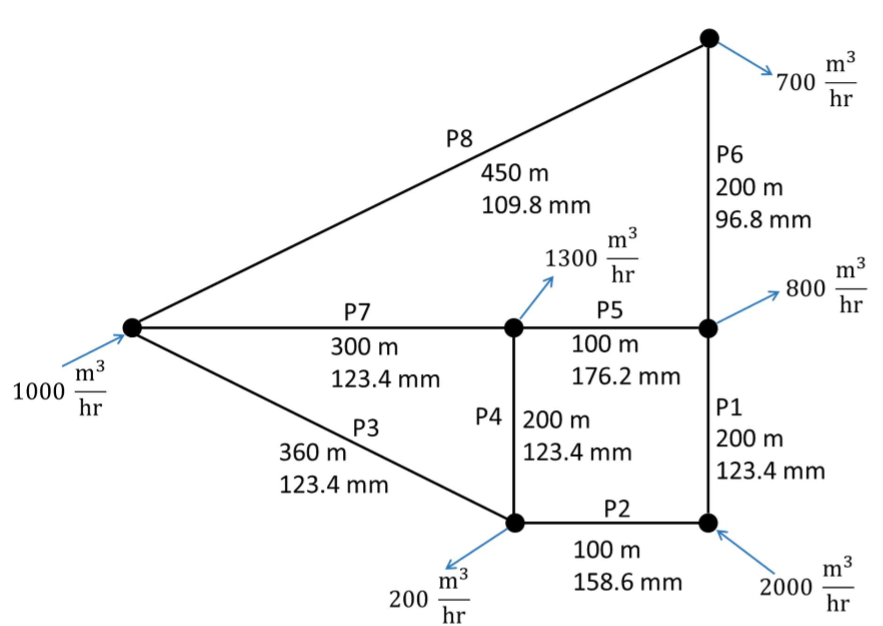
\includegraphics[width=0.6\textwidth]{pics/network.png}
    \caption{Pipe network with three loops}
    \label{pipe}
\end{figure}

By applying conservation of mass through each node, we arrive at the initial guess for the direction and magnitude of the flowrates $Q_j$ through each pipe $j$:

\begin{figure}[h]
    \centering
    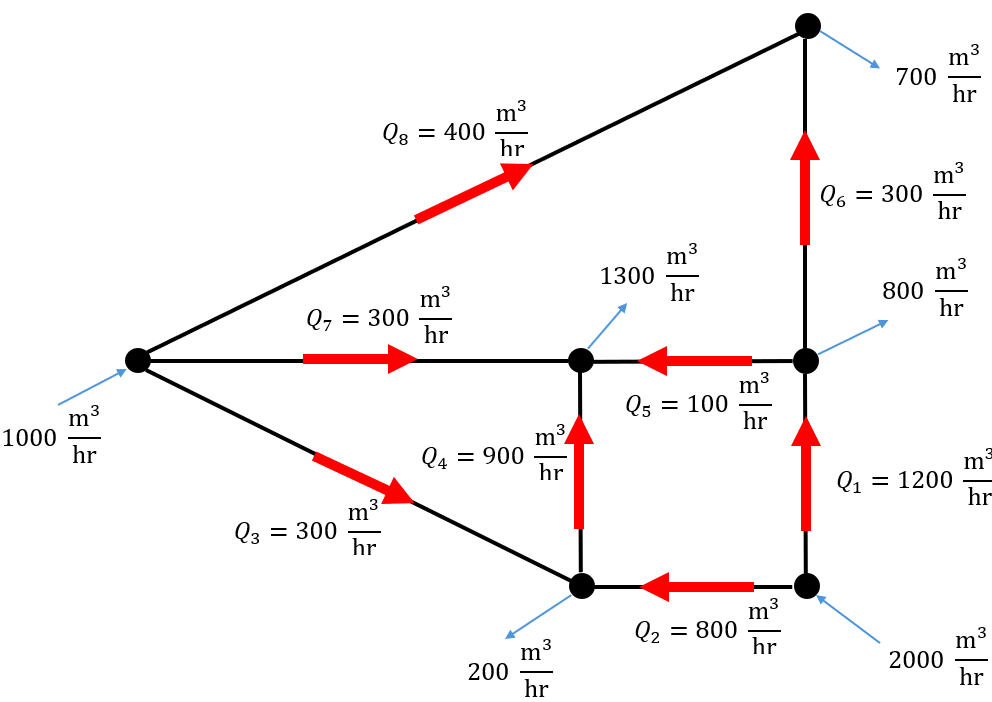
\includegraphics[width=0.71\textwidth]{pics/network2.png}
    \caption{Updated pipe network}
    \label{pipe2}
\end{figure}

\pagebreak

\subsection{Loop and Node Equations}

Labeling each loop and node:

\begin{figure}[h]
    \centering
    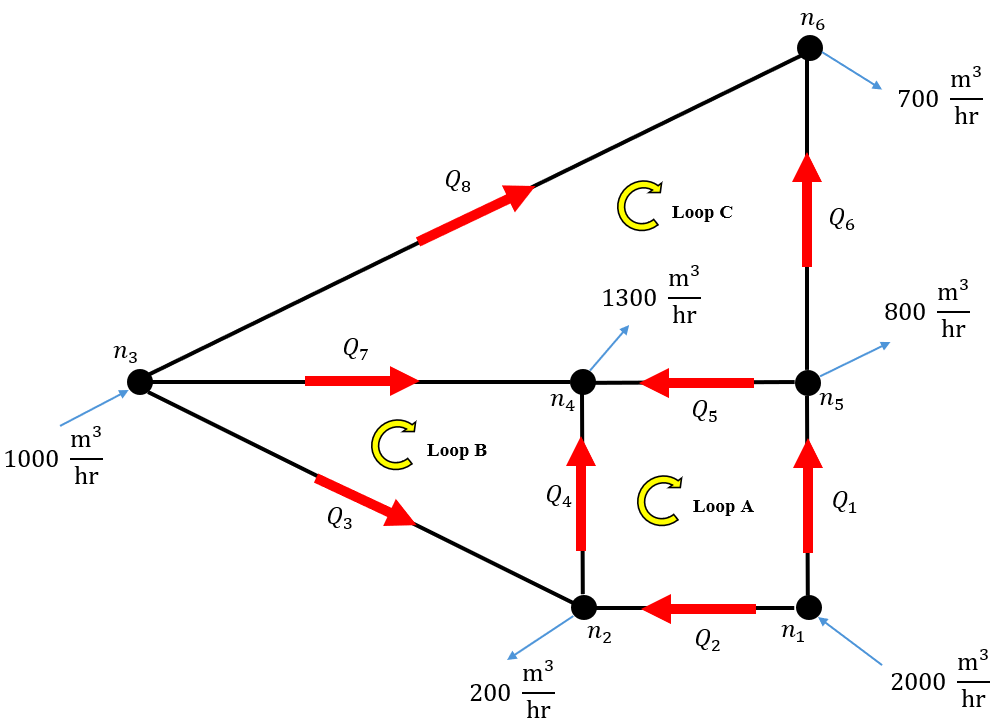
\includegraphics[width=0.8\textwidth]{pics/network3.png}
    \caption{Updated network with loops and nodes labeled}
    \label{pipe3}
\end{figure}

Using Figure~\ref{pipe3} and applying both mass conservation at each node and conservation of energy, we arrive at the 5 node and 
3 loop equations, yielding 8 total:
\begin{tcolorbox}[colback=red!5!white,colframe=red!50!black,title=Solution -- (\textbf{Note}: Flowrates are in $\mathrm{m^3/hr}$)]
    \vspace{-\baselineskip}
    \begin{align*}
        F_1 &= Q_1 + Q_2 - 2000 \\
        F_2 &= Q_3 + Q_7 + Q_8 - 1000 \\
        F_3 &= -Q_4 -Q_5 - Q_7 + 1300 \\
        F_4 &= -Q_1 + Q_5 + Q_6 + 800 \\
        F_5 &= -Q_6 -Q_8 + 700 \\
        F_6 &= -\Darcy{1} + \Darcy{2} + \Darcy{4} - \Darcy{5} \\
        F_7 &= -\Darcy{4} - \Darcy{3} + \Darcy{7} \\
        F_8 &=  \Darcy{5} - \Darcy{6} - \Darcy{7} + \Darcy{8}
    \end{align*}
\end{tcolorbox}

The goal is to search for \textbf{Q} -- a column vector containing the flowrates in each branch -- such that $\textbf{F}(\textbf{Q})=0$, where 
\textbf{F} is a vector-valued function -- containing the set of non-linear algebraic equations -- evaluated at \textbf{Q}.
My MATLAB code \lstinline[style=matlabstyle]|RootFinder_P2.m| uses this
set of non-linear equations, and the other parameters given in Problem 2, to solve for the flowrates using the 
modified-secant method. 


\end{document}
